\section{Digitālās ekonomikas un savienojamības indekss}
\paragraph{}
Latvija DESI 2018. gada rangā ieņem 19. vietu, kas pēdējos divus gadus saglabājusies
nemainīga. Tādējādi valsts attīstības līmenis atbilst ES vidējam. Progresu ļāvuši panākt
uzlabojumi savienojamības aspektā (salīdzinoši augsts ir gan ātrdarbīgu platjoslas tīklu
pārklājuma, gan to izvēršanas līmenis) un digitālo publisko pakalpojumu jomā (Latvijas
Atvērto datu portāla atklāšana, kā arī pēc dažādām dzīves situācijām veidota pieeja, kas
pieņemta publisko pakalpojumu sniegšanas vajadzībām). Aizvien vairāk latviešu izmanto
internetbankas un e-pārvaldes pakalpojumus, taču pusei iedzīvotāju nav digitālo prasmju vai
to līmenis ir zems. Iedzīvotāju digitālo prasmju uzlabošana ir priekšnosacījums, lai varētu
izveidot iekļaujošus darba tirgus, kā arī paaugstināt to uzņēmumu produktivitāti, kuri patlaban
visai maz izmanto digitālās priekšrocības.
\paragraph{}
Latvija pieder pie to valstu grupas, kuru rezultāti ir vidēji.
\paragraph{}
2013. gadā valdība pieņēma Informācijas sabiedrības attīstības pamatnostādnes 2014.–
2020. gadam – pašreizējo nacionālo digitalizācijas stratēģiju. Pamatnostādnes balstītas uz
septiņiem pīlāriem: IKT izglītība un prasmes, plaši pieejama piekļuve internetam, moderna
un efektīva valsts pārvalde, sabiedrībai pieejami e-pakalpojumi un digitālais saturs,
pārrobežu sadarbība digitālā satura vienotajā tirgū, pētniecība un inovācija IKT jomā,
uzticēšanās un drošība.

%example plot
\textit{The \LaTeX\ Companion} book \cite{latexcompanion}
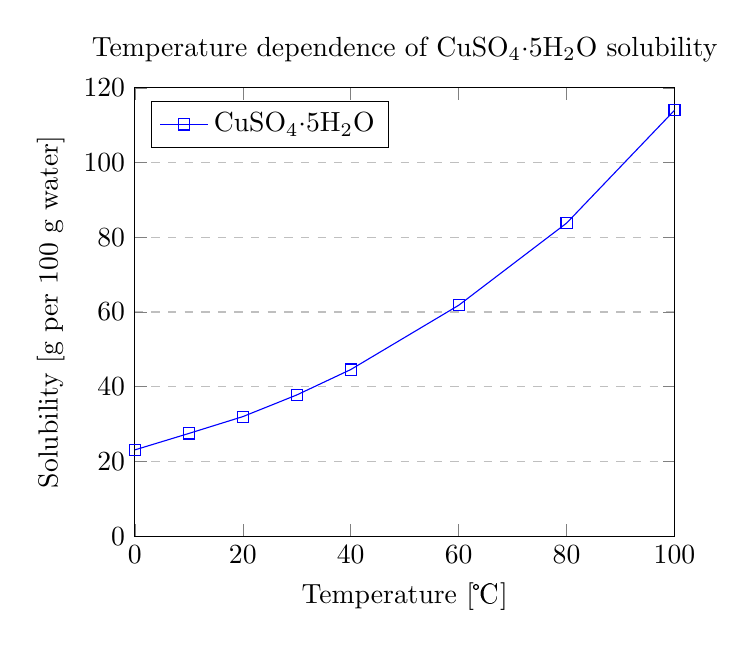
\begin{tikzpicture}
    \begin{axis}[
        title={Temperature dependence of CuSO$_4\cdot$5H$_2$O solubility},
        xlabel={Temperature [\textcelsius]},
        ylabel={Solubility [g per 100 g water]},
        xmin=0, xmax=100,
        ymin=0, ymax=120,
        xtick={0,20,40,60,80,100},
        ytick={0,20,40,60,80,100,120},
        legend pos=north west,
        ymajorgrids=true,
        grid style=dashed,
    ]
     
    \addplot[
        color=blue,
        mark=square,
        ]
        coordinates {
        (0,23.1)(10,27.5)(20,32)(30,37.8)(40,44.6)(60,61.8)(80,83.8)(100,114)
        };
        \legend{CuSO$_4\cdot$5H$_2$O}
     
    \end{axis}
\end{tikzpicture}